%%%%%%%%%%%%%%%%%%%%%%%%%%%%%%%%%%%%%%%%%%%%%%%%%%%%%%%%
%%%%%%%%%%%%%%%%%%%%%%%%%%%%%%%%%%%%%%%%%%%%%%%%%%%%%%%%
%%%%%%%%%%%%%%%%%%%%%%%%%%%%%%%%%%%%%%%%%%%%%%%%%%%%%%%%
\chapter{Classification}
\label{chap:class}

%%%%%%%%%%%%%%%%%%%%%%%%%%%%%%%%%%%%%%%%%%%%%%%%%%%%%%%%
%%%%%%%%%%%%%%%%%%%%%%%%%%%%%%%%%%%%%%%%%%%%%%%%%%%%%%%%
\section{Logistic Regression}
\label{class:logistic}

Logistic regression is a simple method to create a classifier,
typically on two classes $y = 0,1$, though multinomial extensions exist.
Its name comes from the use of the logit, or log-odds, function

\begin{equation}\label{eq:logistic:logic}
l = \text{logit}\left(p\right) = \log\left(\frac{p}{1-p}\right)
\end{equation}

\noindent on the probability $p$ of class $1$.
$l$ is estimated linearly from $n$ input features $x_{j}$ with $n+1$ parameters $\beta_{j}$ as:

\begin{equation}\label{eq:logistic:logicBeta}
l = \beta_{0} + \sum_{j=1}^{n} \, \beta_{j}\,x_{j}\,.
\end{equation}

\noindent The probability $p$ is then

\begin{equation}\label{eq:logistic:p}
p = \frac{e^l}{e^l + 1} = \frac{1}{1+e^{-l}} = \text{logit}^{-1}\left(l\right)
\end{equation}

\noindent which can be turned into a predicted class through the choice of a suitable decision threshold.

The model parameters $\vb*{\beta}$ are chosen by maximizing
the log of the likelihood $L$ \cref{eq:logistic:L} over $m$ known example points $\vb{x}_{i}, y_{i}$.
Note that $P\left(y \mid x\right)$ \cref{eq:logistic:Pr} is simply the Bernoulli distribution.
In practice the log-likelihood $\log\left(L\right)$ is maximized via gradient descent.
An example of logistic regression can be found in \cref{fig:logistic_regression_ex}.

\begin{subequations} \label{eq:logistic:L_Pr}
\begin{align}
L\left(\vb*{\beta} \mid \vb{x}\right) &= \prod_{i=1}^{m} \, P\left(y_{i} \mid \vb{x}_{i};\,\vb*{\beta}\right) \label{eq:logistic:L} \\
P\left(y \mid \vb{x}\right) &= p^y\left(1-p\right)^{1-y}, \quad y \in \{0, 1\} \label{eq:logistic:Pr}
\end{align}
\end{subequations}

\begin{figure}
\centering
% 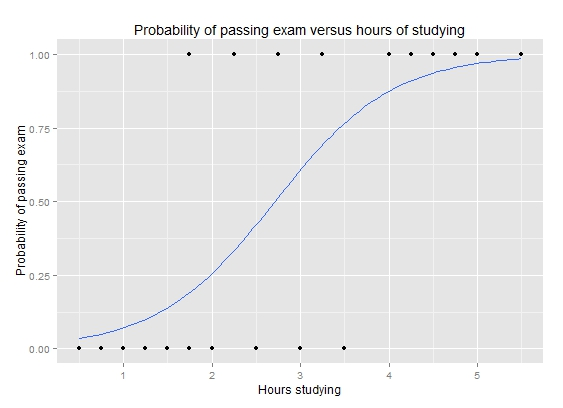
\includegraphics[width=0.8\textwidth]{figures/regression/Exam_pass_logistic_curve.jpeg}
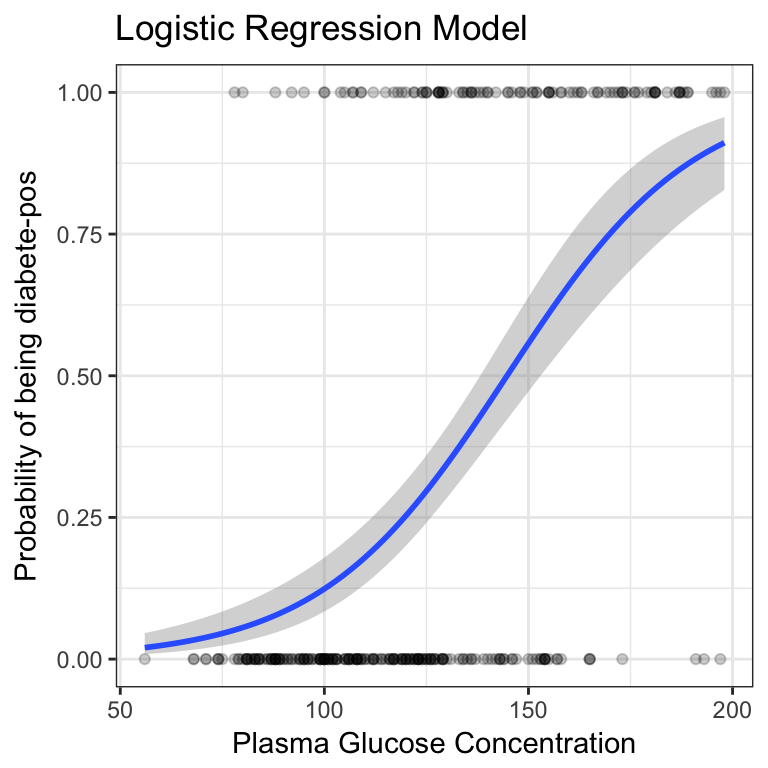
\includegraphics[width=0.7\textwidth]{figures/regression/logistic-regression-probabilities-curve.png}
\caption{
% Example logistic regression curve on one input feature, by \href{https://en.wikipedia.org/wiki/File:Exam_pass_logistic_curve.jpeg}{Michaelg2015}.
Example logistic regression curve on one input feature, by \href{http://www.sthda.com/english/articles/36-classification-methods-essentials/151-logistic-regression-essentials-in-r/}{Kassambara}.
}
\label{fig:logistic_regression_ex}
\end{figure}

%%%%%%%%%%%%%%%%%%%%%%%%%%%%%%%%%%%%%%%%%%%%%%%%%%%%%%%%
\subsection{Assumptions}
\label{class:logistic:assumptions}
% TODO

% TODO any more assumptions?
Some assumptions of the logistic regression approach are:
\begin{enumerate}[noitemsep]
  \item $y$ is either present or absent (dichotomous).
  \item There are minimal correlations between the $x_{j}$ features (no multicollinearity).
  \item There are no major outliers in the data.
\end{enumerate}

% TODO pseudo R2, Wald statistic
% TODO regularized versions?

%%%%%%%%%%%%%%%%%%%%%%%%%%%%%%%%%%%%%%%%%%%%%%%%%%%%%%%%
\subsection{Example}
\label{class:logistic:example}
% TODO

%%%%%%%%%%%%%%%%%%%%%%%%%%%%%%%%%%%%%%%%%%%%%%%%%%%%%%%%
%%%%%%%%%%%%%%%%%%%%%%%%%%%%%%%%%%%%%%%%%%%%%%%%%%%%%%%%
\section{N{a\"i}ve Bayes Classification}
\label{class:Bayes}
% TODO
% TODO maximum a posteriori (italics) probability (MAP) estimator

%%%%%%%%%%%%%%%%%%%%%%%%%%%%%%%%%%%%%%%%%%%%%%%%%%%%%%%%
\subsection{Gaussian N{a\"i}ve Bayes Classification (GNB)}
\label{class:Bayes:GNB}
% TODO

%%%%%%%%%%%%%%%%%%%%%%%%%%%%%%%%%%%%%%%%%%%%%%%%%%%%%%%%
%%%%%%%%%%%%%%%%%%%%%%%%%%%%%%%%%%%%%%%%%%%%%%%%%%%%%%%%
\section{Support Vector Machines (SVM)}
\label{class:SVM}

Basic support vector machines (SVM) work by finding a hyperplane in the $n$-dimensional
feature space of the training data which best separate the different classes.
This is done by maximizing the margin, $2/\norm{\vb{w}}$,
around the hyperplane defined by $\innerproduct{\vb{w}}{\vb{x}} - b = 0$,
where $\innerproduct{\vb{a}}{\vb{b}}$ is the inner product.
For the separable case, as shown in \cref{fig:svm_sep}, this
can be done by minimizing $\norm{\vb{w}}$, with the hard-margin condition that
$y_{i} \left(\innerproduct{\vb{w}}{\vb{x}_{i}} - b\right)$ for all $1 \leq i \leq m$.

However, in reality the data are frequently inseparable and we must switch
to a soft-margin objective function \cref{eq:svm:soft_margin_obj}.
A hinge loss function is included to penalize points on the ``wrong'' side of the margin
proportionally to their distance from the margin.
Here the $\lambda$ hyperparameter sets the tradeoff between
margin size and ensuring points land on their correct sides.

\begin{equation} \label{eq:svm:soft_margin_obj}
S\left(\vb{w}, b\right) =
\lambda\, \norm{\vb{w}}^{2}
+ \frac{1}{m} \sum_{i=1}^{m} \,
\max{\big(0,\, 1 - y_{i} \left(\innerproduct{\vb{w}}{\vb{x}_{i}} - b\right)\big)}.
\end{equation}

\begin{figure}[H]
\centering
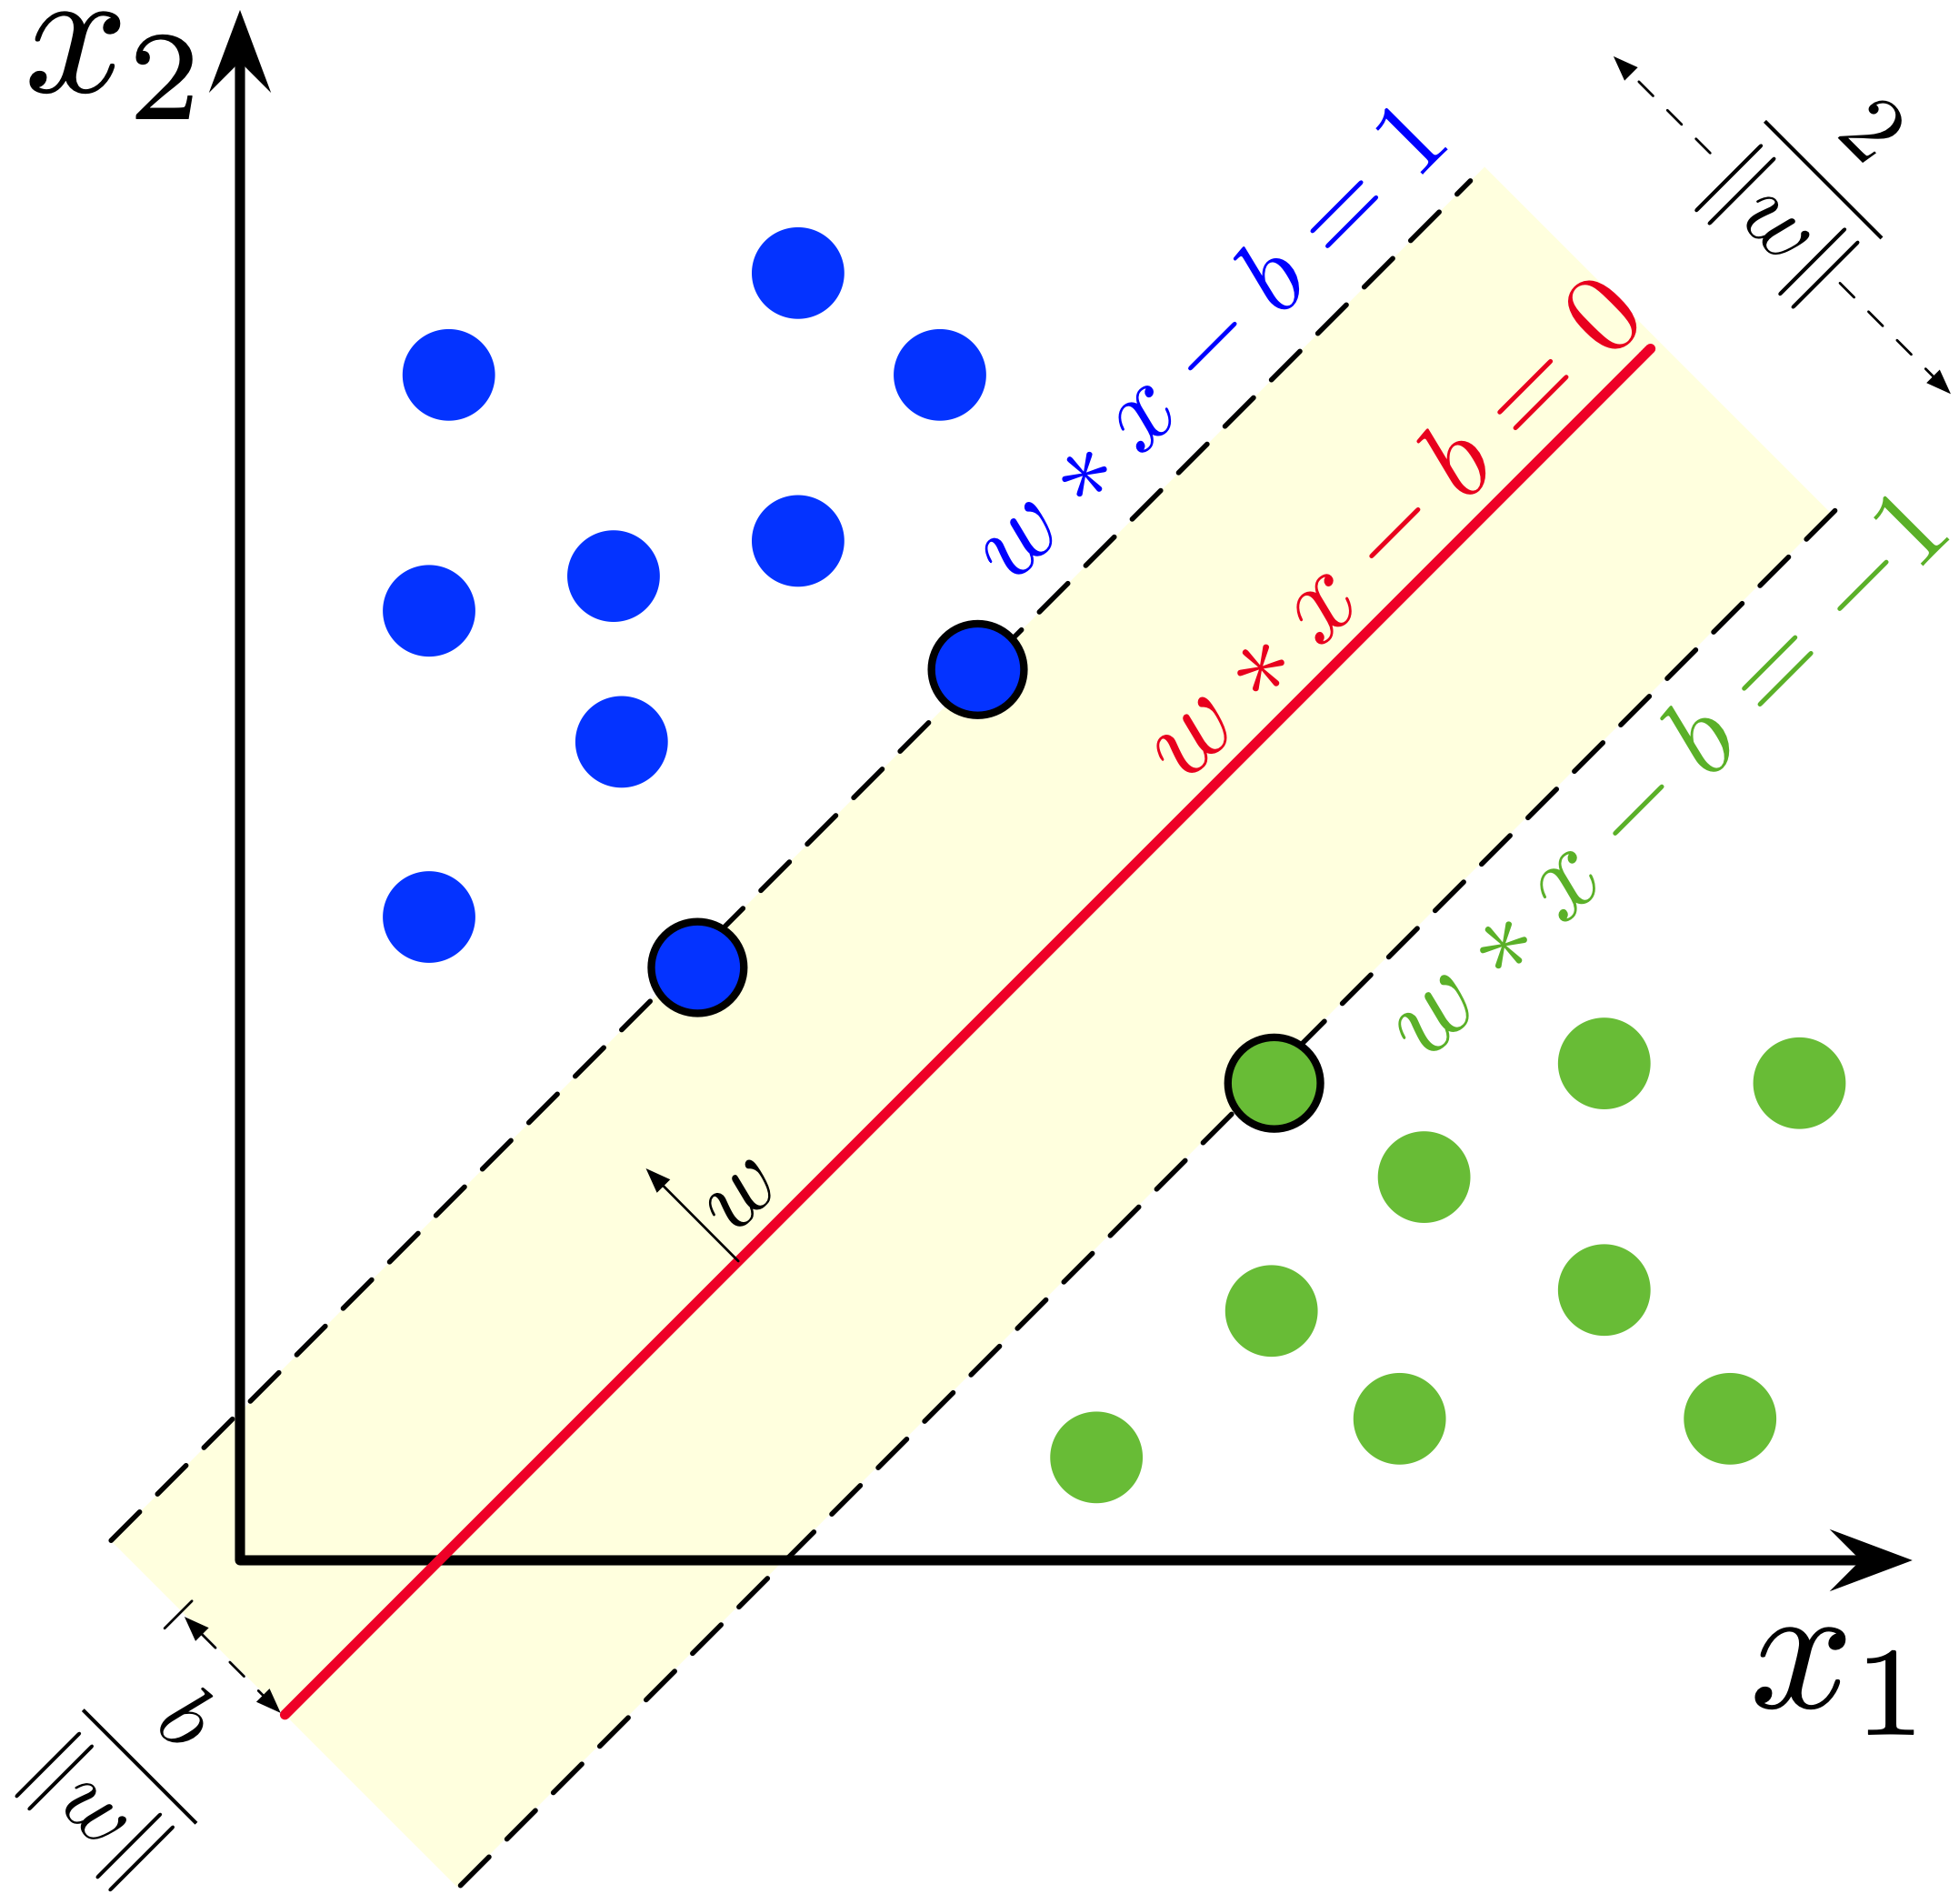
\includegraphics[width=0.42\textwidth]{figures/ml/svm_margin.png}
\vspace{0.2cm}
\caption{
Illustration of the SVM method in the separable case,
by \href{https://en.wikipedia.org/wiki/File:SVM_margin.png}{Larhmam}.
The trained hyperplane in red separates the two classes by the largest margin.
The data points on the margin boundary with black boarders
are known as support vectors, since out of all the data
they are the points really fixing the hyperplane and margin.
}
\label{fig:svm_sep}
\end{figure}

To gain better performance still, we can recast the problem in
a new higher dimensional space where the classes may be easier to separate with a hyperplane.
Fortunately, we do not even need to fully specify the new space,
just a non-linear kernel function\footnote{Common kernel choices include
polynomials of the inner product,
the Gaussian radial basis function,
and the hyperbolic tangent.} $k\left(\vb{a},\vb{b}\right)$
in place of the standard inner product. This is known as the kernel trick.
The classification boundary in the original feature space can then become non-linear,
as can be seen in \cref{fig:svm_kernel_trick}.

\vspace{-0.3cm}% TODo hard coded to fit on one page

\begin{figure}[H]
\centering
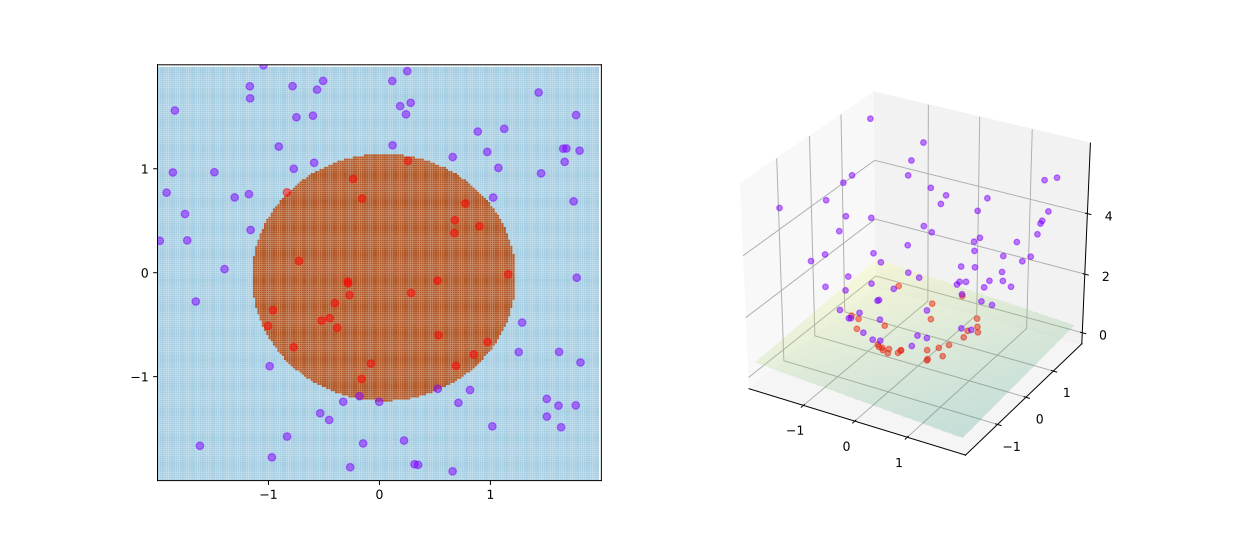
\includegraphics[width=0.8\textwidth,trim={4.0cm 0.8cm 4.0cm 1.4cm},clip]{figures/ml/kernel_trick_example.png}% trim={<left> <lower> <right> <upper>}
\caption{
Graphical example of the kernel trick, by \href{https://en.wikipedia.org/wiki/File:Kernel_trick_idea.svg}{Shiyu Ji}.
Here the kernel $k\left(\vb{a},\vb{b}\right) = \innerproduct{\vb{a}}{\vb{b}} + \norm{\vb{a}}^{2} \norm{\vb{b}}^{2}$
transforms the red and purple classes, linearly inseparable in $n=2$ dimensions on the left,
to a separable $3$-dimensional space on the right.
}
\label{fig:svm_kernel_trick}
\end{figure}

In practice minimizing $S\left(\vb{w}, b\right)$ can be
performed more readily by instead solving the Lagrangian dual problem,
which is computationally efficient to solve with quadratic programming algorithms.
Other modern techniques developed to tackle large and sparse data include
sub-gradient methods and coordinate descent\footnote{Sub-gradient methods work better for large $m$,
coordinate descent for large $n$.}.
However, compared to other classifiers SVM training times
tend to slow significantly for large datasets,
in \sklearn\footnote{See the
\href{https://scikit-learn.org/stable/modules/generated/sklearn.svm.SVC.html}{documentation}
for \texttt{sklearn.svm.SVC}.
\texttt{LinearSVC} may be faster.
The best performance I've seen quoted is $\order{n m \log{\left(m\right)}}$.} by
at least $\order{m^{2}}$, limiting $m \sim \num{e4}$.

%\begin{figure}[H]
%  \centering
%  \begin{subfigure}[b]{0.48\textwidth}\centering
%      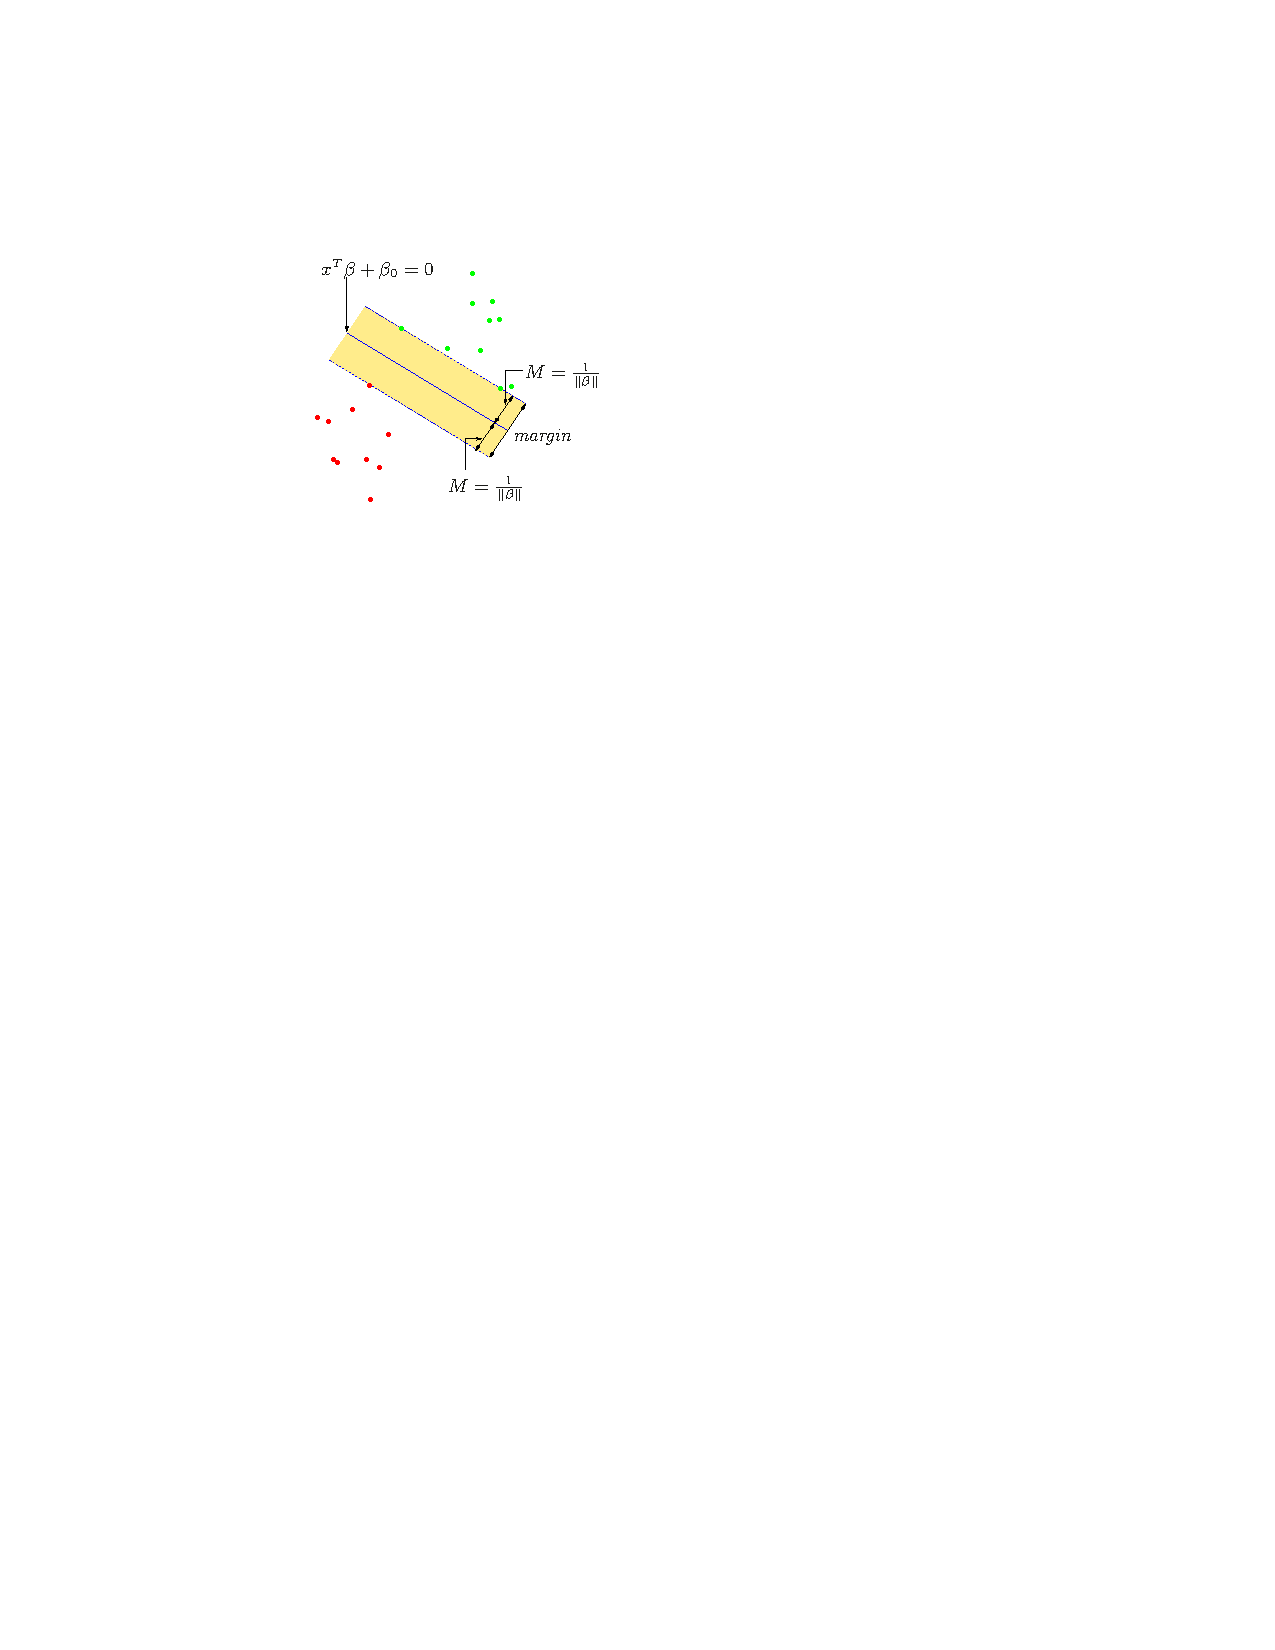
\includegraphics[width=\textwidth]{figures/ml/svm_separable}
%  \caption{Separable}
%  \label{fig:svm:separable}
%  \end{subfigure}
%  ~
%  \begin{subfigure}[b]{0.48\textwidth}\centering
%      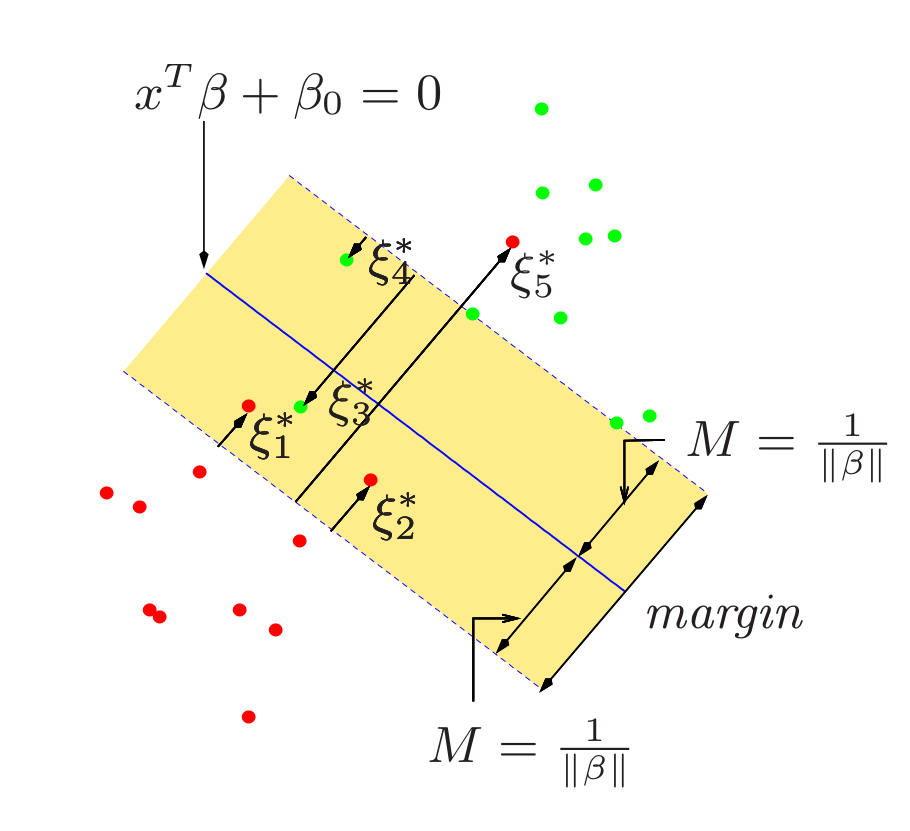
\includegraphics[width=\textwidth]{figures/ml/svm_nonseparable}
%  \caption{Nonseparable}
%  \label{fig:svm:nonseparable}
%  \end{subfigure}
%\caption{
%Illustrations of SVMs in the separable and nonseparable case \cite{HastieTF09}.
%\label{fig:svm}
%}
%\end{figure}

%%%%%%%%%%%%%%%%%%%%%%%%%%%%%%%%%%%%%%%%%%%%%%%%%%%%%%%%
%%%%%%%%%%%%%%%%%%%%%%%%%%%%%%%%%%%%%%%%%%%%%%%%%%%%%%%%
\section{Decision Trees, \texorpdfstring{\ie}{ie} Classification and Regression Trees (CART)}
\label{class:CART}

A basic classifier can be created from a tree of selections on $\mb{X}$ designed to
separate the classes at each branch.
Such a model is known as a classification and regression tree (CART) \cite{Breiman:2253780},
and a simple example can be found in \cref{fig:small_example_CART}.
As the splits are just binary inequality statements on the input variables,
they are --- somewhat --- possible to understand,
and conveniently do not need any kind of feature scaling, unlike other methods.
CART, as the name suggests,
and the tree models of \cref{class:BDT,class:RF,class:FIGS} built on top of it,
can also be used for regression with a suitable choice of splitting criterion,
though we will focus on classification here for brevity.

\begin{figure}[H]
\centering
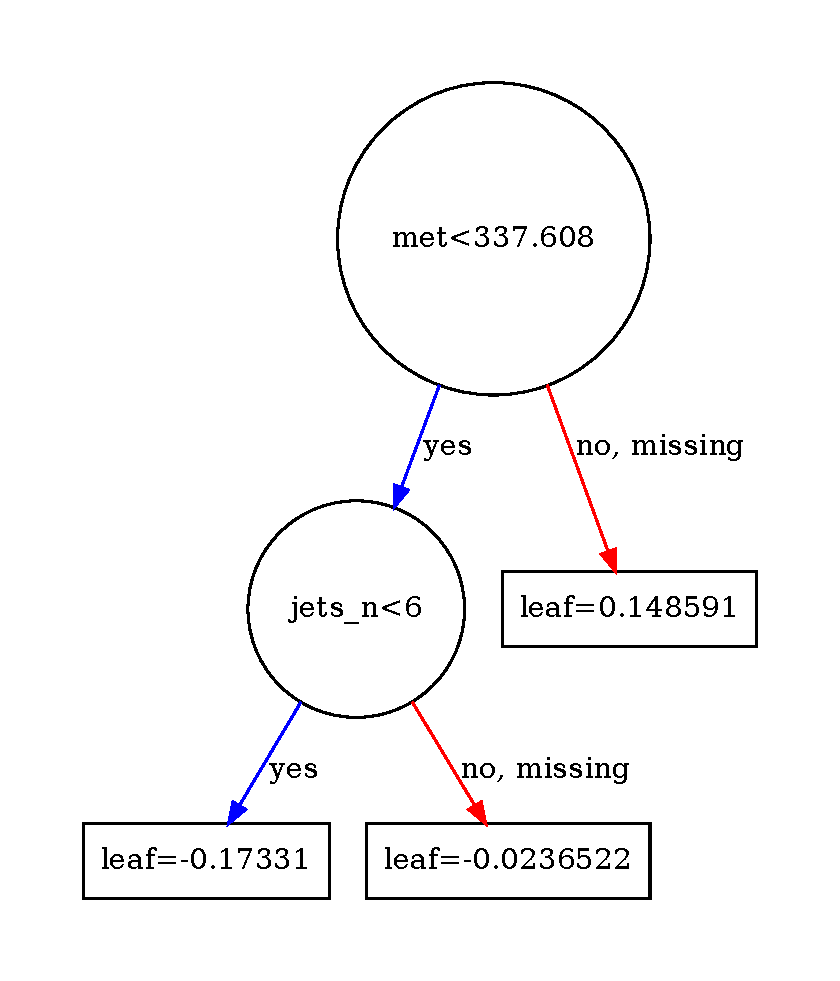
\includegraphics[width=0.4\textwidth]{figures/ml/tree7_g2000_n1200}
\caption{
Simple classification and regression tree (CART) on \num{2} variables
extracted from a \xgboost \cite{XGBoost} model in \cite{mepland_dissertation}.
Here signal-like (background-like) events receive positive (negative) weights in the leaves.
A logistic function is used to properly transform $w$ into a prediction
$\yhat = 1 /\left(1+e^{-w}\right)$ within $0 < \yhat < 1$.
}
\label{fig:small_example_CART}
\end{figure}

%%%%%%%%%%%%%%%%%%%%%%%%%%%%%%%%%%%%%%%%%%%%%%%%%%%%%%%%
\subsection{CART Training}
\label{class:CART:train}

CART models are almost always trained with greedy, \ie local, optimizers
that iteratively grow the tree from a root node.
At each node the optimal split $x_{j} < \beta_{\text{threshold}}$
over the $n$ available features is chosen according to a prespecified splitting criterion.
For classification trees, common choices for the splitting criterion are
the Gini impurity of \cref{class:CART:gini_impurity}
and information entropy of \cref{class:CART:info_entropy},
while the $\text{MSE} = \expval{\left(y-\yhat\right)^{2}}$ is used for regression trees.
In all three cases the optimal split maximizes the decrease, \ie the gain, of the relevant metric.
The tree is constructed in this manner until no additional splits are possible or
halting conditions set by hyperparameters are met, such as
a minimum decrease in splitting criterion,
or a minimum number of training points $\vb{x}_{i}$ in a leaf.

%%%%%%%%%%%%%%%%%%%%%%%%%%%%%%%%%%%%%%%%%%%%%%%%%%%%%%%%
\subsection{Gini Impurity}
\label{class:CART:gini_impurity}

The Gini impurity, or Gini index,
is the probability of incorrectly labeling a randomly selected element of set $S$,
when the label is chosen randomly according to the distribution of labeled elements in $S$.
Letting $p_{k}$ represent the proportion of elements labeled $k$ in $S$,
and $K$ represent the total number of distinct labels in $S$,
the Gini impurity\footnote{In binary classification with $K=2$,
$p_{0} = 1 - p_{1} \, \to \, \text{Gini} = 2 p_{1} \left(1-p_{1}\right)$.} is then:

\begin{equation} \label{eq:gini_impurity}
\text{Gini} = \sum_{k=0}^{K-1} p_{k}\left(1-p_{k}\right) = 1 - \sum_{k=0}^{K-1} p_{k}^{2}\,.
\end{equation}

When $S$ only contains a single label, $K=1$,
the Gini impurity obtains its minimum value of $0$;
any other ``impure'' $S$ will have $0 < \text{Gini} < 1$.
The maximum value of $\text{Gini} = 1-1/K$ occurs when $p_{k} = 1/K, \, \forall k$.

%%%%%%%%%%%%%%%%%%%%%%%%%%%%%%%%%%%%%%%%%%%%%%%%%%%%%%%%
\subsection{Information Entropy}
\label{class:CART:info_entropy}

The information entropy $H$ is a measure of the average
information contained in a random variable's potential outcomes.
In the context of using $H$ as an impurity measurement while growing a CART
over $K$ possible classes we have

\begin{equation} \label{eq:info_entropy_cart}
H = -\sum_{k=0}^{K-1} p_{k} \ln\left(p_{k}\right) \, ,
\end{equation}

\noindent where any ``empty'' classes with $p_{k}=0$
at a given node are ignored in the sum over $k$.
See \cref{misc:info_theory} for additional details on $H$.
Like Gini impurity, the minimum $H = 0$ occurs when $K=1$, with $0 < H$ otherwise.
It can be \href{https://scikit-learn.org/stable/modules/tree.html#classification-criteria}{shown} \cite{sklearn}
that using $H$ while training a CART is equivalent to minimizing
the binary logistic loss function of \cref{ml_general:loss_func:binary_logistic}.

%%%%%%%%%%%%%%%%%%%%%%%%%%%%%%%%%%%%%%%%%%%%%%%%%%%%%%%%
\subsection{Gini Impurity versus Information Entropy}
\label{class:CART:gini_vs_info_entropy}

Using a Taylor expansion\footnote{$\ln\left(1-x\right) = -\sum_{n=1}^{\infty} \frac{x^{n}}{n}$,
where $\abs{x} < 1$ and $x \to 1-p$.
The expansion can be derived directly,
or quickly shown by integrating \cref{eq:misc:math:geometric}.
Note, $0 < p_{k} \leq 1$ in $H$ by construction.} we can rewrite $H$ as

\begin{equation} \label{eq:info_entropy_expanded}
\begin{aligned}
H &= -\sum_{k=0}^{K-1} p_{k} \ln\left(p_{k}\right)\, , \\
&= -\sum_{k=0}^{K-1} p_{k} \left(
-\left(1-p_{k}\right)
-\sum_{n=2}^{\infty} \frac{1}{n}\left(1-p_{k}\right)^{n} \right)\, , \\
&= \text{Gini} + \sum_{k=0}^{K-1} \sum_{n=2}^{\infty} \frac{p_{k}}{n} \left(1-p_{k}\right)^{n}\, ,
\end{aligned}
\end{equation}

\noindent to show that the Gini impurity is simply the lowest order term of the information entropy.
As one would expect from this result,
$\text{Gini}$ and $H$ are very similar functions,
as shown in \cref{fig:gini_vs_info_entropy}
and verified empirically in many CART applications.
In a dedicated study, only \SI{2}{\percent} of optimal splits
disagreed between the two split criteria \cite{Raileanu2004}.
In practice, either criteria can be used without much concern\footnote{There
are some \href{https://ekamperi.github.io/machine\%20learning/2021/04/13/gini-index-vs-entropy-decision-trees.html}{empirical suggestions} that
$H$ may work better with imbalanced classes where $p_{1} \ll 1$ and $\text{Gini} < H$,
see \cref{fig:gini_vs_info_entropy}.
In these cases, just try both criteria.},
however $H$ is slightly slower computationally
as it involves a calculating a $\log$ function.

\begin{figure}[H]
\centering
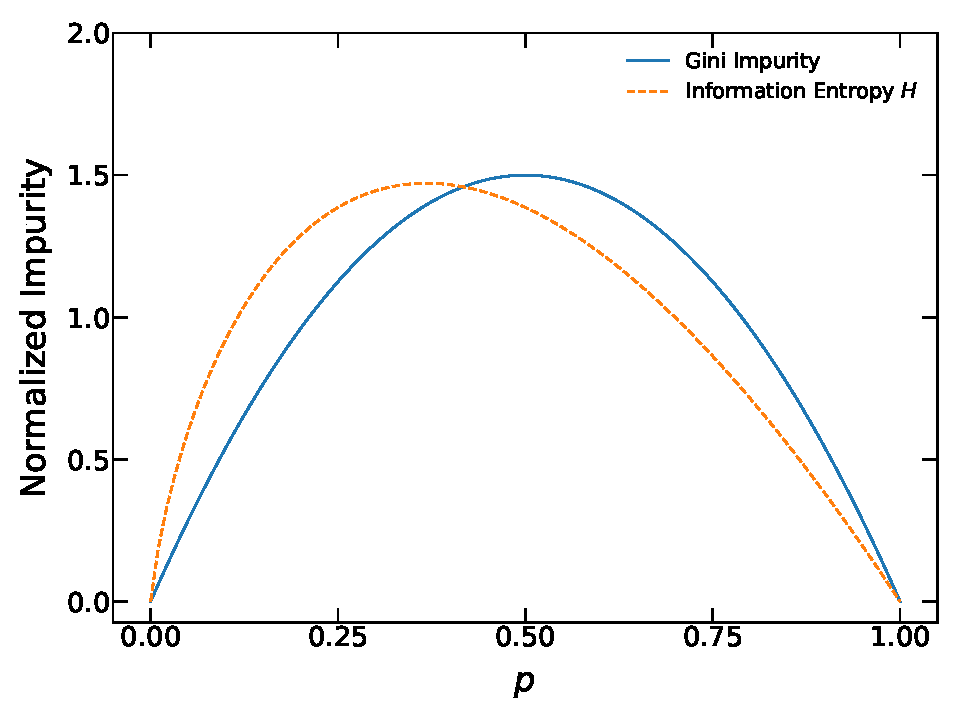
\includegraphics[width=0.5\textwidth]{figures/ml/gini_vs_info_entropy}
\caption{
Gini impurity $\text{Gini} \sim p\left(1-p\right)$ and
information entropy $H \sim p \ln\left(p\right)$
versus $p$, normalized to unit area.
Both metrics are quite similar,
with $H$ being slightly biased toward smaller $p$.
}
\label{fig:gini_vs_info_entropy}
\end{figure}

%%%%%%%%%%%%%%%%%%%%%%%%%%%%%%%%%%%%%%%%%%%%%%%%%%%%%%%%
\subsection{CART Predictions}
\label{class:CART:pred}

To make a prediction for data point $\vb{x}_{i}$
the tree and its branches are traversed until a leaf is reached.
The prediction assigned by the leaf can be constructed in a few ways;
a class label may be assigned directly based on the majority class in the leaf during training,
a probability can be assigned based on the proportion of classes in the leaf,
or a weight $w$ can be computed from the loss function and training data in a more complex manner,
\eg \cref{class:BDT:xgboost,class:FIGS}.
Note that the leaf weights can be trained separately from the tree structure
using an independent fold of the training data.
Tree models trained with this approach are known as ``honest'' \cite{JMLR:v13:biau12a,pmlr-v32-denil14}.

%%%%%%%%%%%%%%%%%%%%%%%%%%%%%%%%%%%%%%%%%%%%%%%%%%%%%%%%
%%%%%%%%%%%%%%%%%%%%%%%%%%%%%%%%%%%%%%%%%%%%%%%%%%%%%%%%
\section{Boosted Decision Tree (BDT)}
\label{class:BDT}

Individual CARTs are rather poor and limited models
in terms of the behaviors they can successfully predict.
However, by taking an ensemble of $K$ complementary trees,
\ie boosting \cite{10.5555/3091696.3091715,FREUND1997119,Breiman1996BiasV,friedman2000} as described in \cref{ml_general:boosting},
and combining each CART's individual predicted weight $w_{k}$
a much more flexible boosted decision tree (BDT) is formed.
The component trees of a BDT are generated by iteratively adding new trees $f_{k}\left(\vb{x}_{i}\right)$ to those which came before \cite{XGBoost},

\begin{equation} \label{eq:boosting}
\begin{aligned}
\yhat^{\left(0\right)} &= 0\,, \\
\yhat^{\left(1\right)} &= f_1\left(\mb{X}\right) = \yhat^{\left(0\right)} + f_1\left(\mb{X}\right), \\
\yhat^{\left(2\right)} &= f_1\left(\mb{X}\right) + f_2\left(\mb{X}\right)= \yhat^{\left(1\right)} + f_2\left(\mb{X}\right), \\
                           &\vdotswithin{\displaystyle =} \\
\yhat^{\left(t\right)} &= \sum_{k=1}^t f_k\left(\mb{X}\right)= \yhat^{\left(t-1\right)} + f_t\left(\mb{X}\right),
\end{aligned}
\end{equation}

\noindent where each tree $f_{k}$ is grown from zero branches while minimizing the objective function $S\left(\beta\right)$.
Through the ingenious use of a second order Taylor expansion this process can
be recast as a form of gradient descent\footnote{See \cite{NIPS1999_96a93ba8} for a different explanation.}, and thus is known as
stochastic gradient boosting \cite{10.2307/2699986,FRIEDMAN2002367}.
The number of boosting rounds, and thus trees, $K$ can be chosen in advance,
but is better optimized during the training process via early stopping.

%%%%%%%%%%%%%%%%%%%%%%%%%%%%%%%%%%%%%%%%%%%%%%%%%%%%%%%%
\subsection{\xgboost}% would rather have the \textsc caps than italics
\label{class:BDT:xgboost}
% TODO see https://towardsdatascience.com/boosting-algorithm-xgboost-4d9ec0207d
% TODO how does the Hessian come into play?
% TODO how are leaf weights $w$ are computed in each tree?
% TODO provide \order for training

The \xgboost\footnote{\xgboost: eXtreme Gradient Boosting, \href{https://github.com/dmlc/xgboost}{github.com/dmlc/xgboost}.} library \cite{XGBoost}
is a modern open source implementation of gradient boosted decision tree methods.
Through various algorithmic and memory optimizations \xgboost demonstrates good performance\footnote{\xgboost has lost
its lead in recent years to newer libraries such as LightGBM \cite{LightGBM}
and CatBoost \cite{CatBoost}, but is still a standard library.}.
L1 and L2 regularization is incorporated via

\begin{equation} \label{eq:bdt_omega_reg}
\Omega\left(f\right) = \alpha T + \frac{1}{2}\lambda \sum_{j=1}^T w_{j}^{2}\,,
\end{equation}

\noindent where $T$ is the number of leaves in a tree and $w_{j}$ are the leaf weights;
however, the default hyperparameters of $\alpha=0$ and $\lambda=1$ only enable L2 regularization.
Other important hyperparameters in \xgboost include the
learning rate $\eta$, which scales the corrections added by each new tree,
maximum tree depth, which sets a limit on the complexity of any tree via its depth,
and the early stopping validation threshold.
For reference $\eta=0.3$ and a maximum depth of 6 are the default values.

%%%%%%%%%%%%%%%%%%%%%%%%%%%%%%%%%%%%%%%%%%%%%%%%%%%%%%%%
\subsection{AdaBoost}
\label{class:BDT:AdaBoost}
% TODO

%%%%%%%%%%%%%%%%%%%%%%%%%%%%%%%%%%%%%%%%%%%%%%%%%%%%%%%%
%%%%%%%%%%%%%%%%%%%%%%%%%%%%%%%%%%%%%%%%%%%%%%%%%%%%%%%%
\section{Random Forest}
\label{class:RF}
% TODO

% TODO (RF)
% TODO best results occur when you chose $\sqrt{n}$ features randomly to build each tree

%%%%%%%%%%%%%%%%%%%%%%%%%%%%%%%%%%%%%%%%%%%%%%%%%%%%%%%%
%%%%%%%%%%%%%%%%%%%%%%%%%%%%%%%%%%%%%%%%%%%%%%%%%%%%%%%%
\section{Fast Interpretable Greedy-Tree Sums (\figs)}
\label{class:FIGS}

Fast Interpretable Greedy-Tree Sums (\figs) \cite{FIGS,G-FIGS}
is an extension of the basic CART structure introduced in \cref{class:CART}.
Depending on the nature of the training data,
a CART will tend to reproduce subsets of the tree along different branches.
The resulting deep trees are not ideal as they contain many splits,
increasing the chance of fitting to noise in the data,
and because they have less data to work with at each subsequent split,
increasing the variance of the tree's predictions.

\figs improves upon the iterative training process of CART
by considering adding the next split as the root of a new tree $f_{t}$,
in addition to adding the next split at the bottom of an existing tree.
This reduces the number of splits when the data has an additive structure,
as can be seen in \cref{fig:FIGS:intro}, thereby also increasing the interpretability.
The splits are chosen greedily according to the usual splitting criteria;
typically the Gini impurity of \cref{class:CART:gini_impurity} is used for classification.

During training, each tree $k$ is fit to the residuals remaining after summing the other tree's predictions,
$r_{i}^{\left(-k\right)}$ \cref{eq:FIGS:FIGS_eqs:r}.
The predicted weight $w_{l,\,k}$ \cref{eq:FIGS:FIGS_eqs:weight} at each leaf $l$ of tree $k$
are found by taking the mean of the $r_{i}^{\left(-k\right)}$ residuals, from the other trees,
over the $\vb{x}_{i}$ data points $\left\{l\right\}$ that reach the leaf.
Note that when there are no other trees,
\eg when growing the first tree or if the data is non-additive,
the sum $\sum_{t \neq k} f_{t}$ will be zero and $r_{i}^{\left(-k\right)} = y_{i}$.
In this case, the leaf weights are simply $w_{l} = n_{l,\,1}/n_{l}$,
\ie the proportion of positive $y_{i} = 1$ data points in leaf $l$.
Finally, the predictions for the trained model are made by
summing the relevant leaf weight $w_{l,k}\left(\vb{x}_{i}\right)$ from each tree.
See \cref{algo:FIGS:fit_algo} for an outline of the training algorithm.

\begin{subequations}\label{eq:FIGS_eqs}
\begin{align}
r_{i}^{\left(-k\right)} &= y_{i} - \sum_{t \neq k} f_{t}\left(\vb{x}_{i}\right) \label{eq:FIGS:FIGS_eqs:r} \\
w_{l,\,k} &= \frac{1}{\abs{\left\{l\right\}}} \sum_{i \in \left\{l\right\}} r_{i}^{\left(-k\right)} \label{eq:FIGS:FIGS_eqs:weight}
\end{align}
\end{subequations}

\begin{figure}[H]
\centering
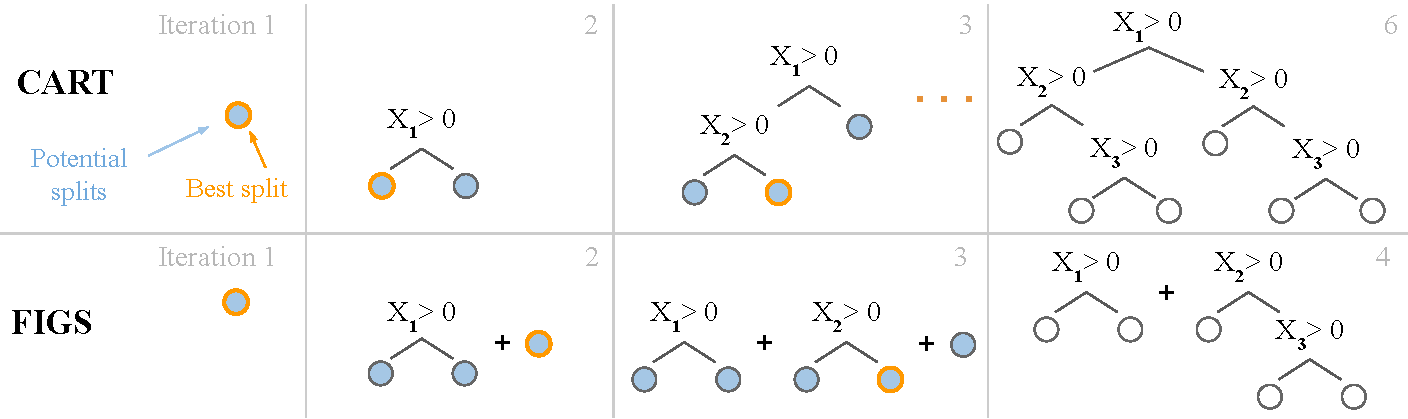
\includegraphics[width=\textwidth]{figures/ml/figs_intro_fig}
\caption{
A comparison of CART and \figs tree growth on the toy dataset
$y = \identity_{x_{1} > 0} + \identity_{x_{2} > 0} \, \identity_{x_{3} > 0}$ \cite{FIGS}.
At each training iteration \figs considers adding a new split at the bottom of the existing tree(s) like CART,
but also considers starting a new tree entirely.
Notice that CART must repeat the $x_{2}, x_{3}$ subtree on each side of the $x_{1}$ split,
while \figs captures the additive structure of $y$ directly, thereby saving \num{2} splits.
}
\label{fig:FIGS:intro}
\end{figure}

\begin{algorithm}[h]
  \caption{\figs fitting algorithm, adapted from \cite{FIGS}.}
  \label{algo:FIGS:fit_algo}
  \small
\begin{algorithmic}
  \State {\figs}(X: features, y: outcomes, $\nu$: max\_splits)
  \State trees = []
  \While{count\_total\_splits(trees) $< \nu$:}
    \State all\_trees = join(trees, build\_new\_tree()) \textcolor{codegreen}{\# add new tree}
    \State potential\_splits = []
    \For{}\hspace{-3pt}tree in all\_trees:
        \State y\_residuals = y $-$ predict(all\_trees except tree)
        \For{}\hspace{-3pt}leaf in tree:
            \State potential\_split = split(X, y\_residuals, leaf)
            \State potential\_splits.append(potential\_split)
        \EndFor
    \EndFor
    \State best\_split = split\_with\_min\_impurity(potential\_splits)
    \State trees.insert(best\_split)
  \EndWhile
\end{algorithmic}
\end{algorithm}

The resulting \figs model is thus an ensemble of CART-like trees,
similar to the BDT and RF models of \cref{class:BDT,class:RF}.
However, \figs can explicitly capture any additive structure present in the data,
while the ensemble trees of the BDT (RF) model being trained sequentially (independently) can not.
Rather than constraining the depth or number of trees separately like other tree-based models,
\figs can impose a limit on the total number of splits across all trees via the hyperparameter $\nu$.
This makes the construction of small, interpretable, models much easier.
Similar to CART, \figs can also set hyperparameters for
the minimum decrease in impurity and
number of features to consider at each split.
With $\nu < 20$, readily interpretable \figs models have been observed
to have state-of-the-art performance on multiple datasets \cite{FIGS}.
A \python implementation of the \figs algorithm can be found in the \texttt{imodels} package \cite{imodels}.
The \figs training time goes as $\order{n \, \nu^{2} m^{2}}$ \cite{FIGS},
where $n$ is the number of features and $m$ is the number of data points,
which is quite fast on a modern machine for reasonable $m$, even when $n$ is large.

A demonstration of \figs versus \xgboost, \cref{class:BDT:xgboost},
on a synthetic dataset containing additive structure
is provided in the \texttt{figs\_demo.ipynb} \href{https://github.com/mepland/data_science_notes/blob/main/plots/figs_demo.ipynb}{notebook}.
Visualizations of the three trees of the trained \figs model can be found in \cref{fig:FIGS:demo_trees}.
The \figs model has $\SI{8.4}{\percent}$ lower performance, as measured by ROC AUC, when compared to the \xgboost model.
However, the \figs model is much more interpretable,
using only \num{30} splits (\num{3} trees) versus \num{1496} splits (\num{64} trees) used by \xgboost,
a reduction of \SI{4887}{\percent} (\SI{2033}{\percent})!

The demonstration training dataset was created from two Monte Carlo (MC) generators, $i=0,1$,
combined with a logical \texttt{AND} on $\vb{y}_{i}$.
The features were labeled $\texttt{x\_i\_j}$ to indicate the originating MC generator.
In this case\footnote{The degree of separation between MC generators
\figs can achieve depends on the random seed and MC parameters.
Values that showed good separation were chosen here to illustrate
the power of \figs on additive data,
but further study is needed to quantify this behavior.},
the \figs model was able to discern the additive structure,
as can be seen by the general separation of the \texttt{x\_i\_j} features by $i$ between the \num{3} trees.
Lastly, with its constrained splits \figs is naturally more regularized than \xgboost,
as can be seen in the ROC curves of \cref{fig:FIGS:demo_roc:figs},
which should lead to less generalization error in production usage.

\newpage

\begin{landscape}
\begin{figure}[H]
  \centering
  \begin{subfigure}[b]{0.32\linewidth}\centering
      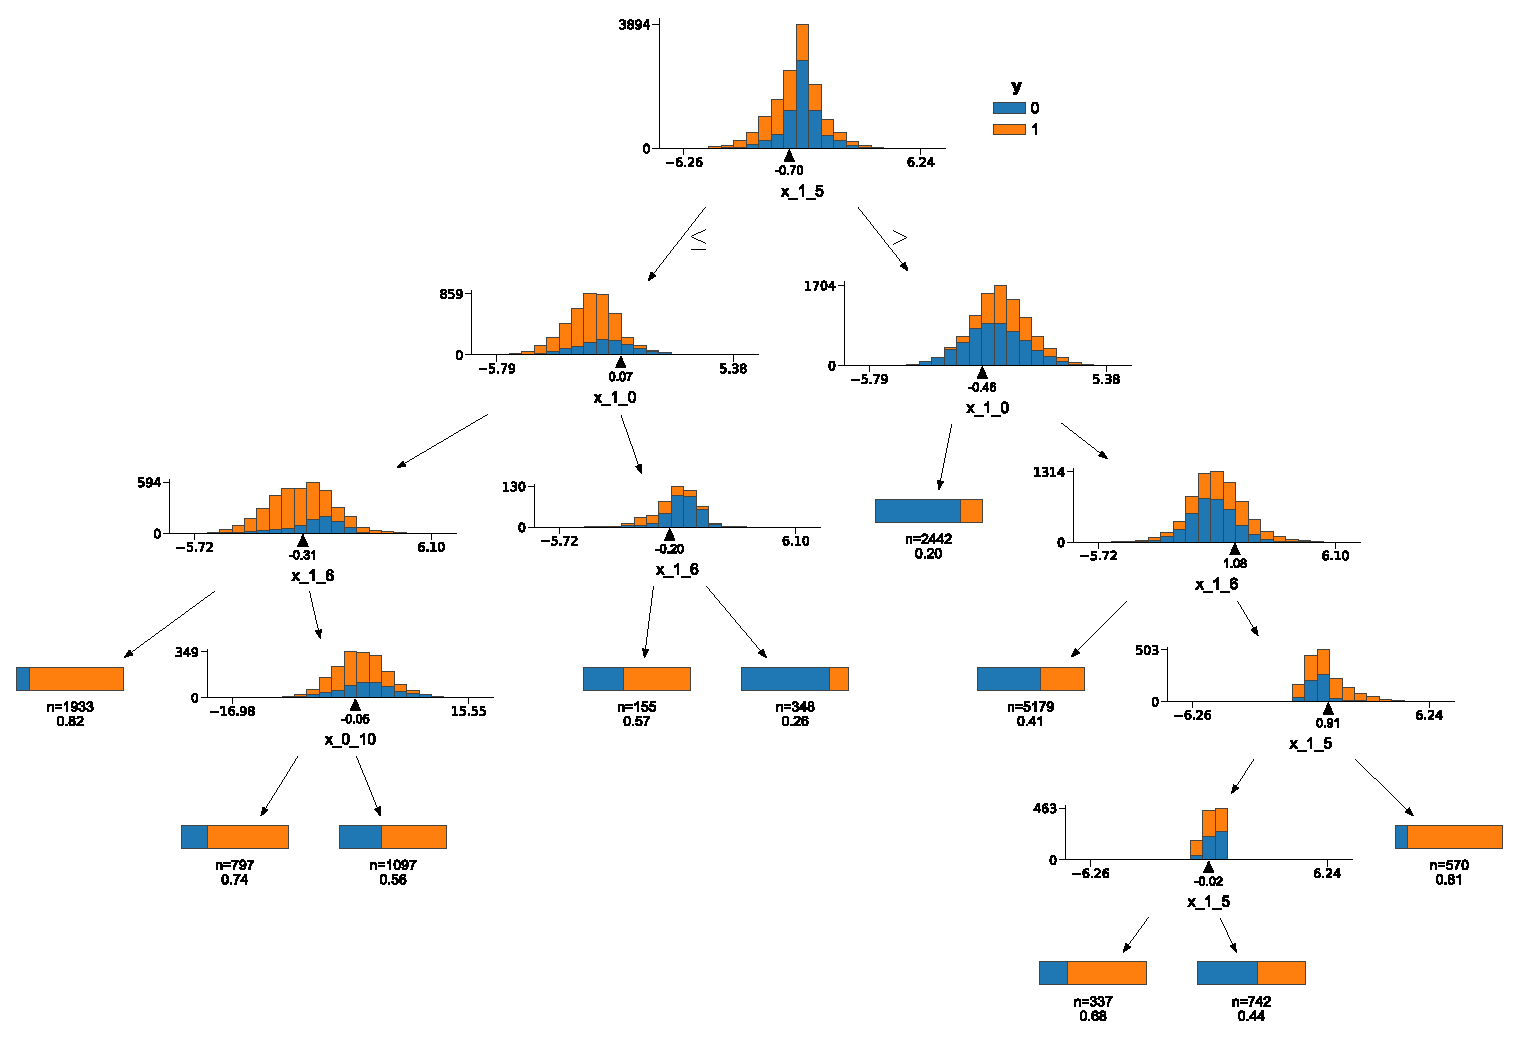
\includegraphics[width=\textwidth]{figures/ml/figs_demo/dtreeviz_figs_0}
  \caption{Tree 0}
  \label{fig:FIGS:demo_trees:tree0}
  \end{subfigure}
  ~
  \begin{subfigure}[b]{0.32\linewidth}\centering
      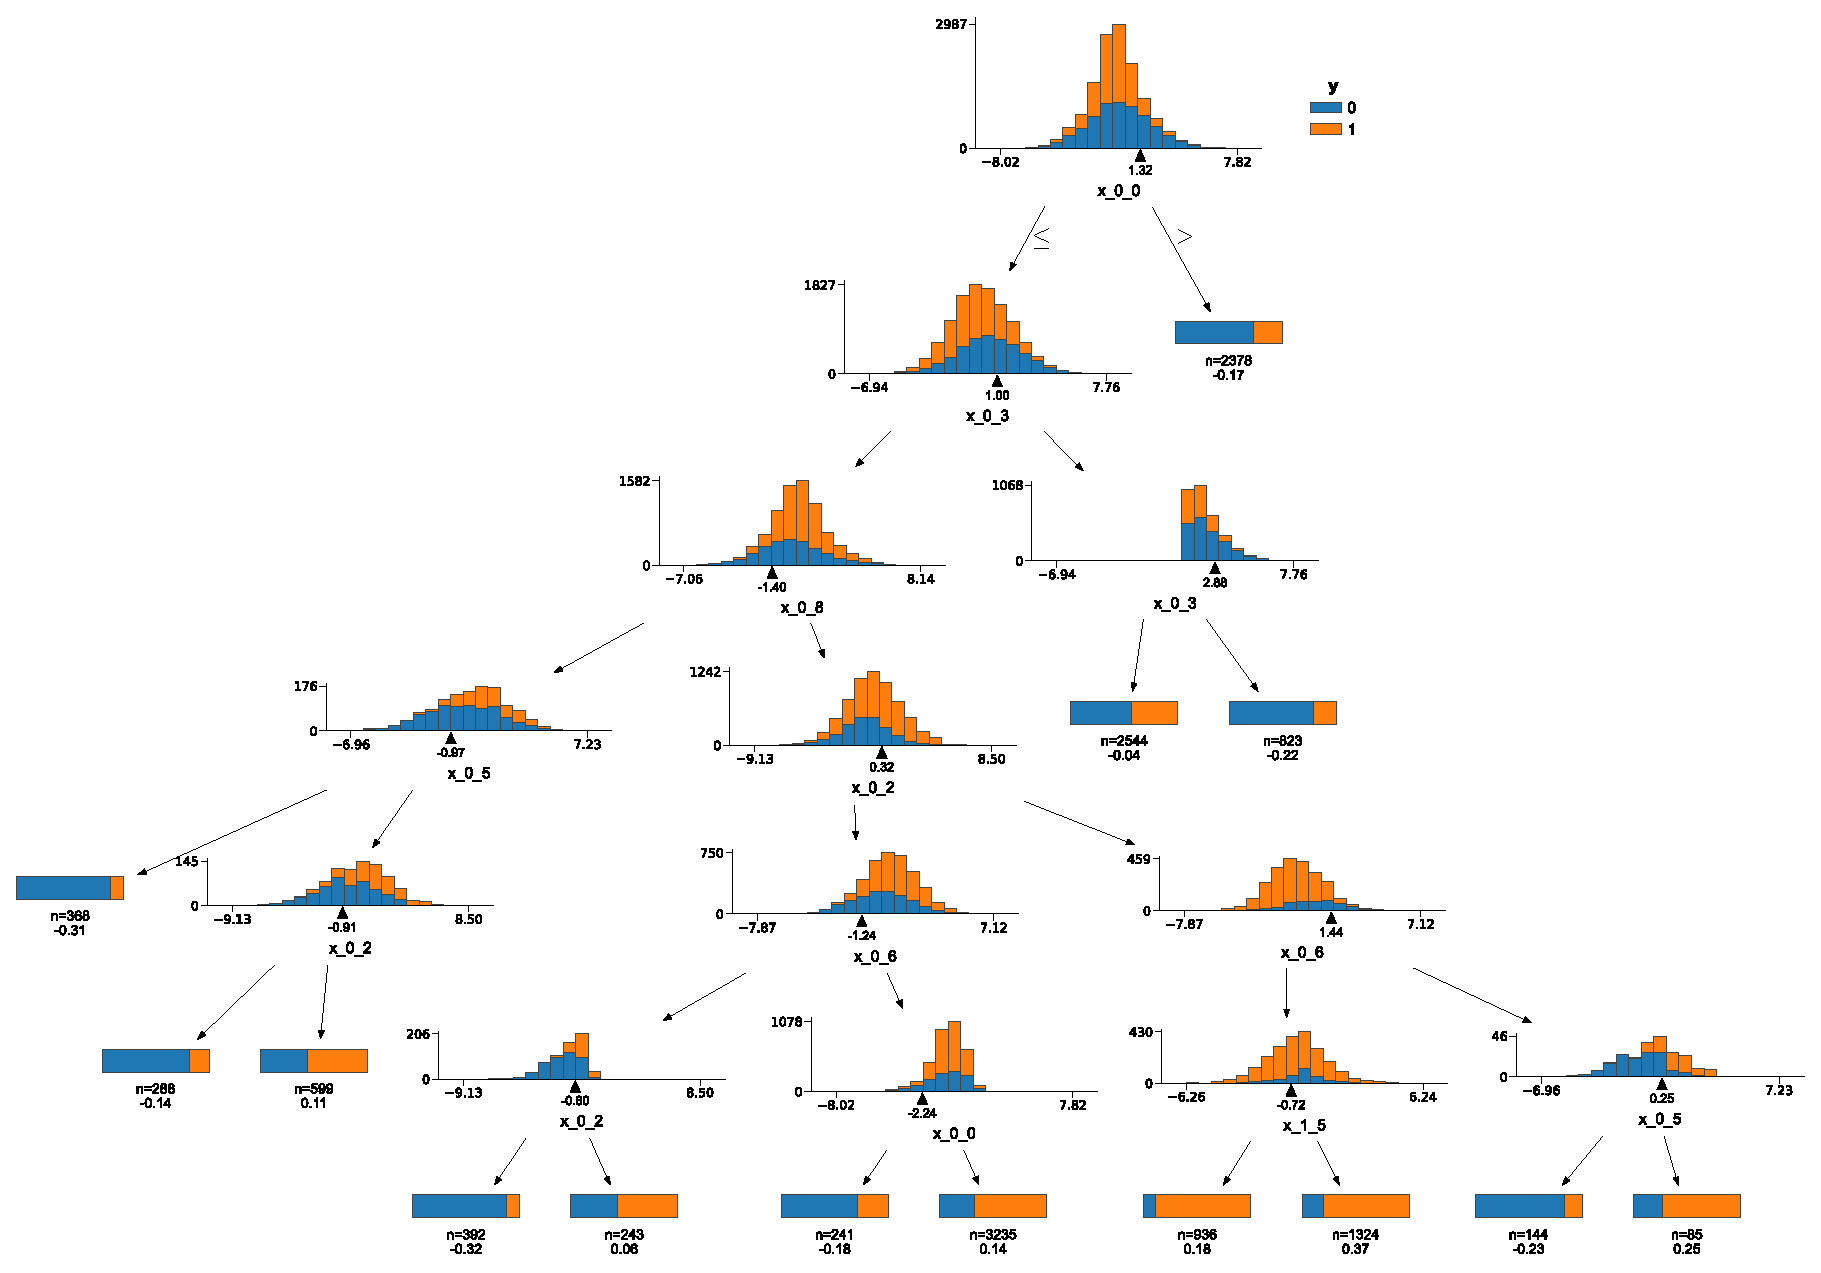
\includegraphics[width=\textwidth]{figures/ml/figs_demo/dtreeviz_figs_1}
  \caption{Tree 1}
  \label{fig:FIGS:demo_trees:tree1}
  \end{subfigure}
  ~
  \begin{subfigure}[b]{0.32\linewidth}\centering
      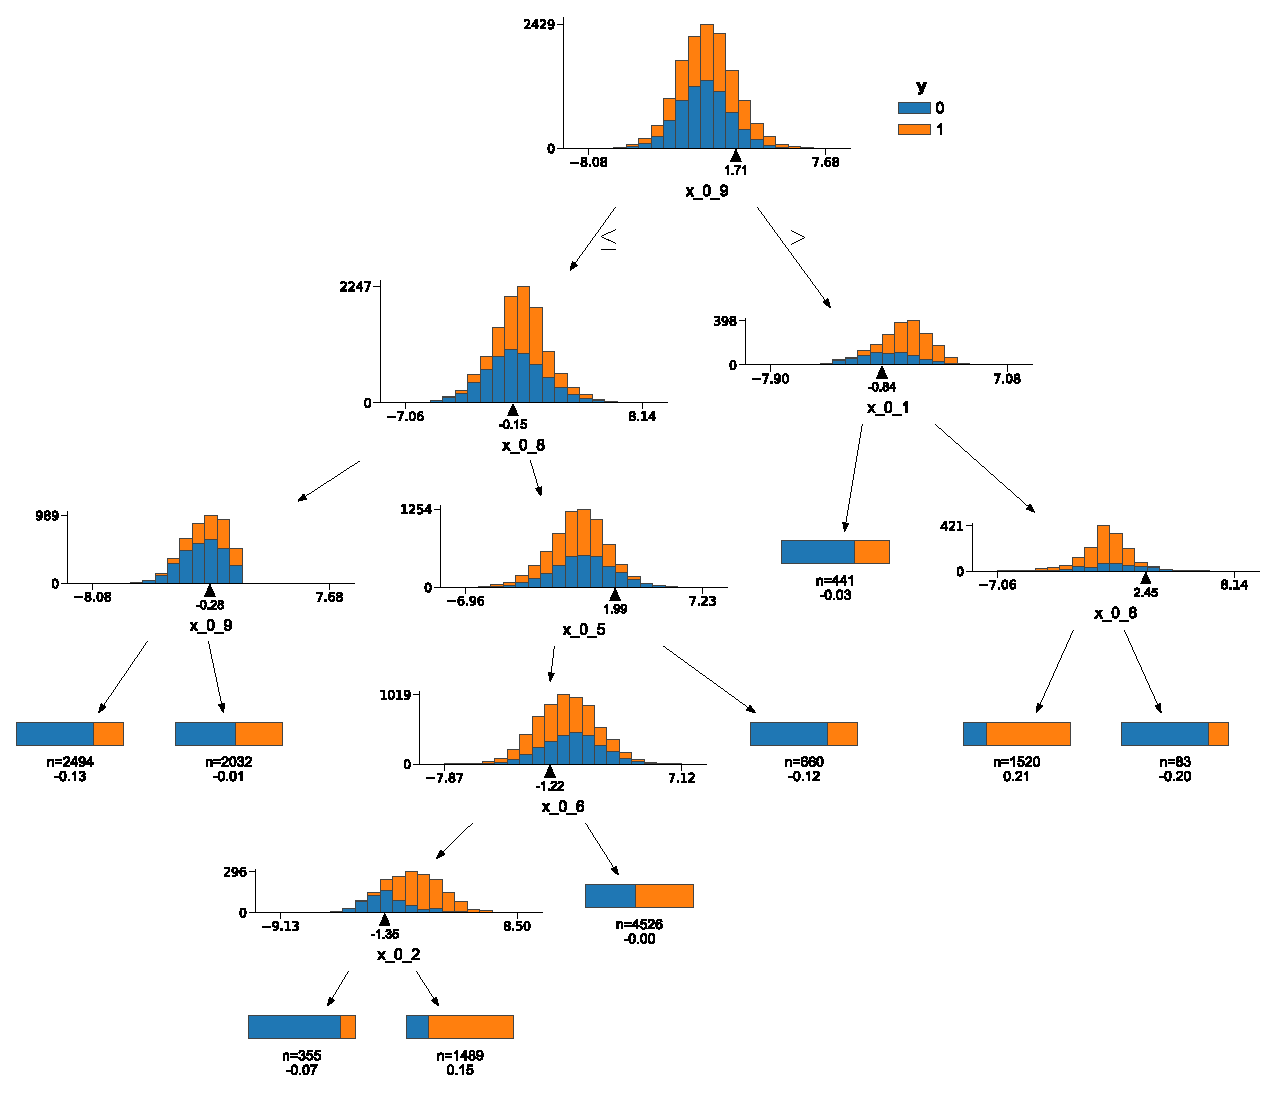
\includegraphics[width=\textwidth]{figures/ml/figs_demo/dtreeviz_figs_2}
  \caption{Tree 2}
  \label{fig:FIGS:demo_trees:tree2}
  \end{subfigure}
\caption{
The \figs model as trained on synthetic data in the
\texttt{figs\_demo.ipynb} \href{https://github.com/mepland/data_science_notes/blob/main/plots/figs_demo.ipynb}{notebook}.
Tree visualizations were created with the \texttt{dtreeviz} \href{https://github.com/parrt/dtreeviz}{package}.
The relatively small number of splits, \num{30}, and trees, \num{3}, make the \figs model readily interpretable.
In this case, the \figs model was able to learn the additive structure of the data,
as can be seen by each tree primarily splitting on a single MC generator $i$,
as shown in the feature names \texttt{x\_i\_j}.
To make predictions for $\vb{x}$, the weights at each terminating node are summed to create $P\left(y=1\right)$.
\label{fig:FIGS:demo_trees}
}
\end{figure}
\end{landscape}

\newpage

\begin{figure}[H]
  \centering
  \begin{subfigure}[b]{0.75\textwidth}\centering
      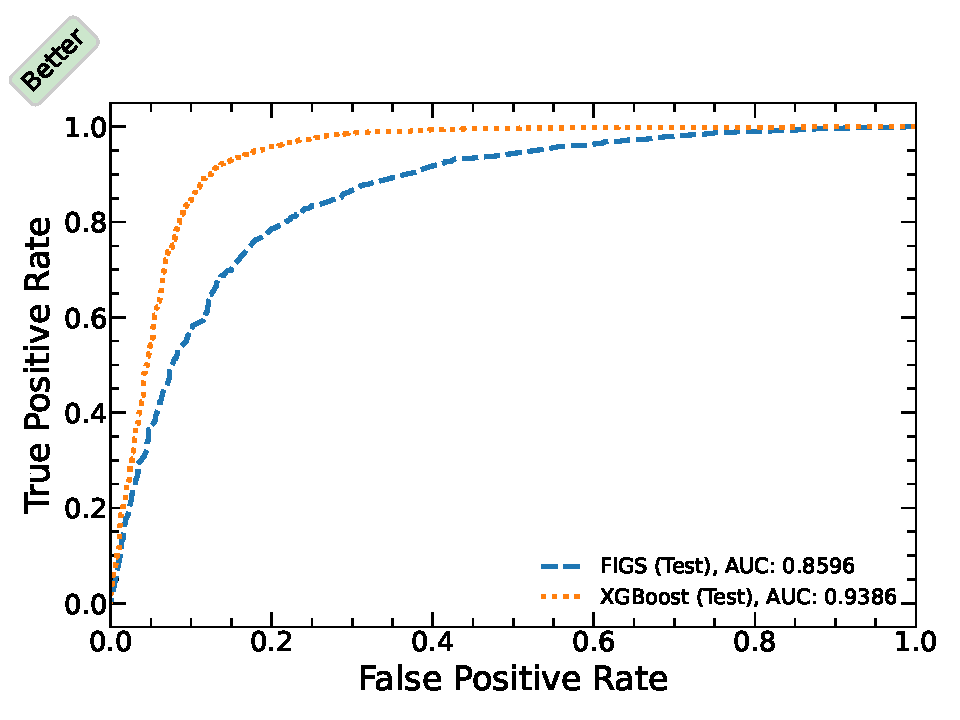
\includegraphics[width=\textwidth]{figures/ml/figs_demo/roc_figs_test_xgboost_test}
  \caption{\figs and \xgboost Test Set Comparison}
  \label{fig:FIGS:demo_roc:figs_xgboost}
  \end{subfigure}
  \newline
  \begin{subfigure}[b]{0.48\textwidth}\centering
      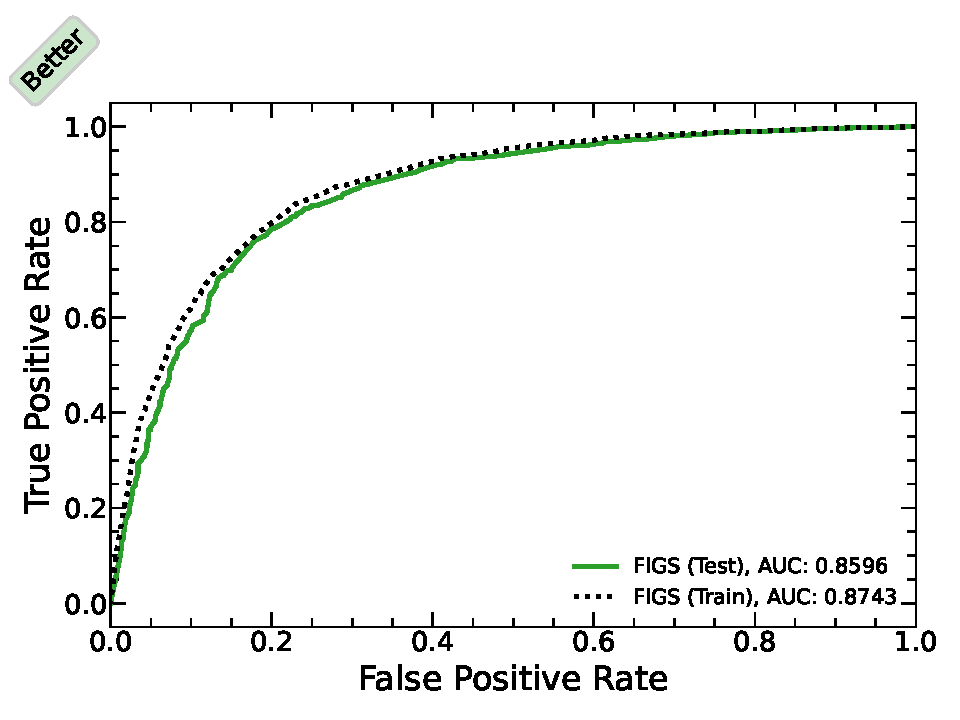
\includegraphics[width=\textwidth]{figures/ml/figs_demo/roc_figs_test_train}
  \caption{\figs}
  \label{fig:FIGS:demo_roc:figs}
  \end{subfigure}
  ~
  \begin{subfigure}[b]{0.48\textwidth}\centering
      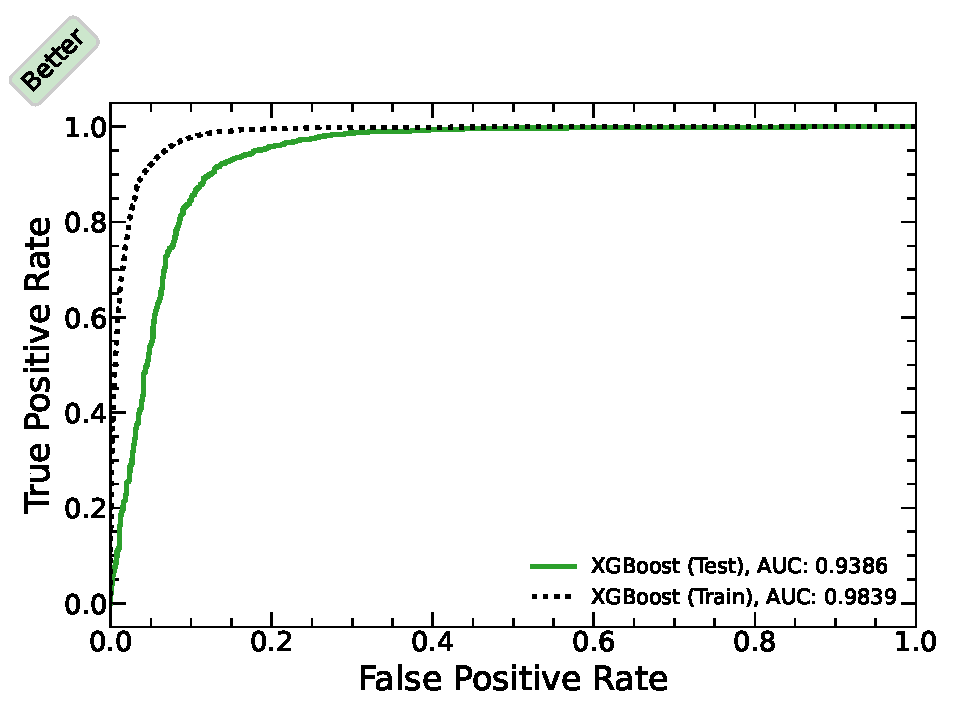
\includegraphics[width=\textwidth]{figures/ml/figs_demo/roc_xgboost_test_train}
  \caption{\xgboost}
  \label{fig:FIGS:demo_roc:xgboost}
  \end{subfigure}
\caption{
ROC curves for the \figs and \xgboost models trained in the
\texttt{figs\_demo.ipynb} \href{https://github.com/mepland/data_science_notes/blob/main/plots/figs_demo.ipynb}{notebook}.
While the \xgboost model has better performance, \mysubref{fig:FIGS:demo_roc:figs_xgboost},
the \figs model is much more interpretable and
is more consistent between train and test set performance, \mysubref{fig:FIGS:demo_roc:figs},
which should lead to less generalization error in production.
\label{fig:FIGS:demo_roc}
}
\end{figure}

%%%%%%%%%%%%%%%%%%%%%%%%%%%%%%%%%%%%%%%%%%%%%%%%%%%%%%%%
%%%%%%%%%%%%%%%%%%%%%%%%%%%%%%%%%%%%%%%%%%%%%%%%%%%%%%%%
\section{\texorpdfstring{$k$}{k}-Nearest Neighbors (\texorpdfstring{$k$}{k}-NN)}
\label{class:kNN}
% TODO
% TODO \kNN

%%%%%%%%%%%%%%%%%%%%%%%%%%%%%%%%%%%%%%%%%%%%%%%%%%%%%%%%
%%%%%%%%%%%%%%%%%%%%%%%%%%%%%%%%%%%%%%%%%%%%%%%%%%%%%%%%
\section{Artificial Neural Networks (NN)}
\label{class:ANN}
% TODO

% TODO add back prop somewhere, here or in grad descent

\begin{figure}[H]
  \centering
  \begin{subfigure}[b]{0.48\textwidth}\centering
      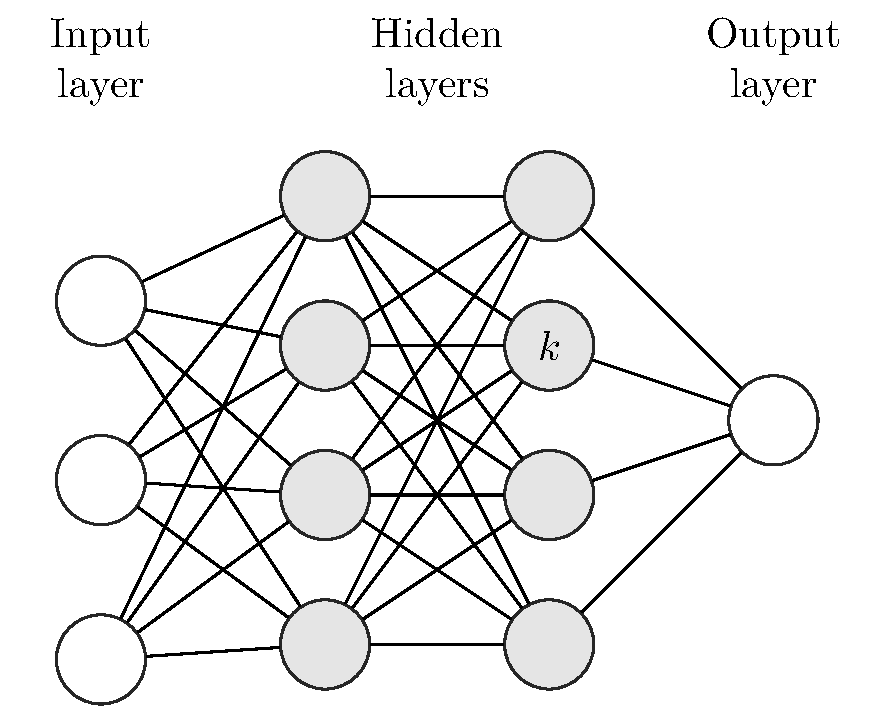
\includegraphics[width=\textwidth]{figures/ml/NN_diagram/NN_diagram}
  \caption{NN Example}
  \label{fig:NN:ex}
  \end{subfigure}
  ~
  \begin{subfigure}[b]{0.48\textwidth}\centering
      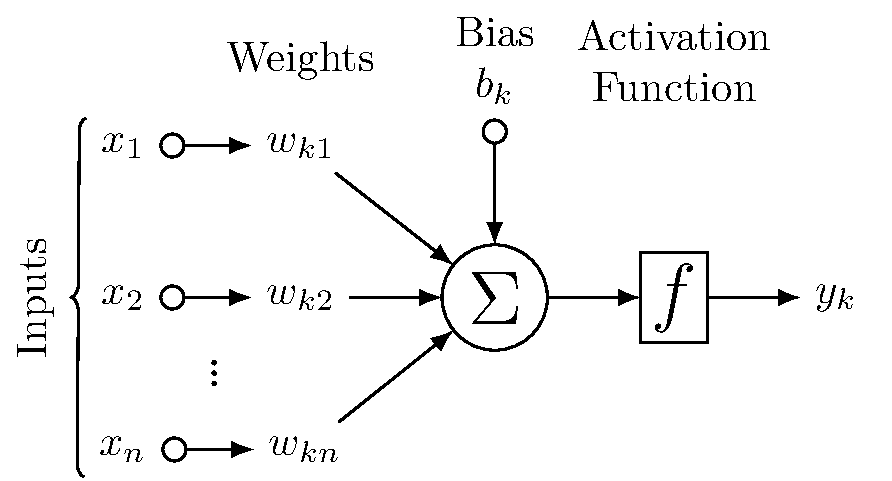
\includegraphics[width=\textwidth]{figures/ml/NN_neuron/NN_neuron}
  \caption{Neuron}
  \label{fig:NN:Neuron}
  \end{subfigure}
\caption{
Illustrations of the components of a neural network.
\label{fig:NN}
}
\end{figure}

%%%%%%%%%%%%%%%%%%%%%%%%%%%%%%%%%%%%%%%%%%%%%%%%%%%%%%%%
%%%%%%%%%%%%%%%%%%%%%%%%%%%%%%%%%%%%%%%%%%%%%%%%%%%%%%%%
\section{Recursive Neural Networks (RNN)}
\label{class:RNN}
% TODO

%%%%%%%%%%%%%%%%%%%%%%%%%%%%%%%%%%%%%%%%%%%%%%%%%%%%%%%%
\subsection{Long Short Term Memory (LSTM)}
\label{class:RNN:LSTM}
% TODO

%%%%%%%%%%%%%%%%%%%%%%%%%%%%%%%%%%%%%%%%%%%%%%%%%%%%%%%%
%%%%%%%%%%%%%%%%%%%%%%%%%%%%%%%%%%%%%%%%%%%%%%%%%%%%%%%%
\section{Convolutional Neural Networks (CNN)}
\label{class:CNN}
% TODO

%%%%%%%%%%%%%%%%%%%%%%%%%%%%%%%%%%%%%%%%%%%%%%%%%%%%%%%%
%%%%%%%%%%%%%%%%%%%%%%%%%%%%%%%%%%%%%%%%%%%%%%%%%%%%%%%%
\section{Learning Vector Quantization (LVQ)}
\label{class:kNN:LVQ}
% TODO

%%%%%%%%%%%%%%%%%%%%%%%%%%%%%%%%%%%%%%%%%%%%%%%%%%%%%%%%
%%%%%%%%%%%%%%%%%%%%%%%%%%%%%%%%%%%%%%%%%%%%%%%%%%%%%%%%
\section{Addressing Class Imbalance}
\label{class:imbalance}
% TODO

TODO \cref{ml_general:eval:class_priors}
